\documentclass[entwurf]{uebblatt}

\begin{document}

\maketitle{7}

\begin{center}
  \emph{Dieses Blatt kommt erst nächste Woche nach der Dienstagsvorlesung heraus.}
\end{center}

\begin{aufgabe}{Verzweigung von Primidealen}
\begin{enumerate}
\item Sei~$K = \QQ[\sqrt[3]{2}]$. Es ist~$(1,\sqrt[3]{2},\sqrt[3]{2}^2)$ eine
Ganzheitsbasis von~$\O_K$. Bestimme das Verzweigungsverhalten der
Primzahlen~$2, 3, 5$ und~$11$ in~$\O_K$.
\item Was möchte dir \emph{Mumfords Schatzkarte} mitteilen? Analysiere sie so
gut wie möglich!

\centering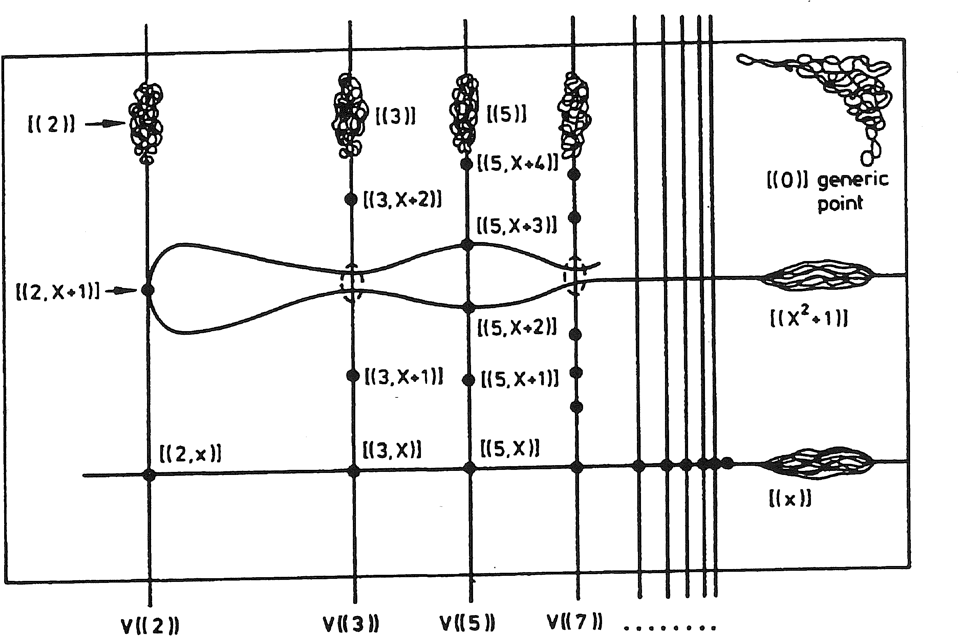
\includegraphics[width=0.7\textwidth]{images/mumfords-treasure-map}
\end{enumerate}
\end{aufgabe}

\end{document}
